\chapter{Background in optimal control problems}
\label{cha:OCP}
This chapter gives some background information on the theory behind optimal control problems (OCP) in section \ref{Optimal control problem (OCP)}. After a global introduction and a discussion about discretization and time shooting methods, this chapter introduces the concept of model predictive control (MPC) in section \ref{s:MPC_e}.

\section{Optimal control problem (OCP)}
\label{Optimal control problem (OCP)}
"An optimal control problem determines the desired inputs and corresponding state trajectories to change the system from an initial state to a desired final state in an optimal way while satisfying input and state constraints." \cite{Mercy2018}.

\begin{equation}
\label{eq:OCP}
\begin{aligned}
\min_{\bm{q},\bm{u}} \quad & \int_{0}^{T}l(\bm{q}(t),\bm{u}(t))dt + E(\bm{q}(T)) \\
\textrm{s.t.} \quad & \bm{\dot{q}}(t) = \bm{f}(\bm{q}(t), \bm{u}(t))\\
& \bm{q}(0)= \bm{q}_{0},\hspace{2 mm}\bm{q}(T)= \bm{q}_{T}    \\
& \bm{q}(t)\in Q,\hspace{3 mm} \bm{u}(t)\in U, \hspace{3 mm} t\in [0, T]
\end{aligned}
\end{equation}

$\bm{q}$ is called the state vector and contains all the states of the system. $\bm{u}$ is the control vector containing the controls. In theory the amount of states of a system can be infinite, but in order to sufficiently model a system only a well chosen set of states is needed. Typical controls $\bm{u}$ for a vehicle are steerwheelangle and the amount of throttle which can be directly linked to the amount of propulsion force. Also higher order controls are possible.\\
The objective function $l$ of the optimization problem Eq. (\ref{eq:OCP}) is integrating over the desired control horizon $T$. In the objective function it is indicated what should be minimized and this is in function of the different states and controls. $E(\bm{q}(T))$ describes the terminal cost and the objective is reduced when the system comes closer to a predefined final state at the end of the control horizon.
The dynamics of the system are modelled by an explicit ordinary differential equation $\bm{\dot{q}}(t) = \bm{f}(\bm{q}(t), \bm{u}(t))$ and the evolution of the vehicle states are retrieved by integrating this ODE over the control horizon.
$Q$ and $U$ represent the feasible space wherein solutions for the OCP can be sought. It is worth noting that the control horizon time $T$ itself can be an optimization variable. What comes out of a OCP indicates what states will be visited by the system and which controls have to be applied in order to optimize the associated objective function with respect to predefined constraints. \cite{Panos_opti}\\ 

There is a difference between soft and hard constraints. A hard constraint directly demarcates the feasible solution spaces $\bm{q}(t)\in Q,\hspace{3 mm} \bm{u}(t)\in U$. A soft constraint is added in the objective function $l$ and will contribute to a more optimal solution when it is better fulfilled. Also when a soft constraint is not met this can be an optimal solution which is not the case for a hard constraint. \cite{Yankov} \\

\subsection{Time discretization}
\label{s:time_dis}
The optimal control problem Eq. (\ref{eq:OCP}) is continuous in time. This means that it has infinite dimensions, but to be able to run the optimization problem on digital systems there is need for discretization. Several ways to do this are available and summarized in Figure Eq. (\ref{fig:discretization_m}).\cite{Gillis2019}
\begin{figure}[htp]
	\centering
	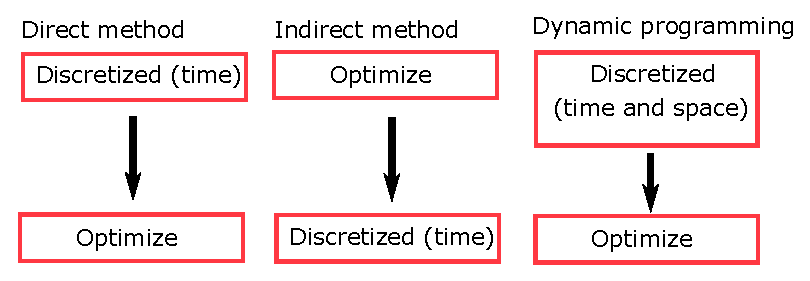
\includegraphics[width=0.8\textwidth]{discretized.eps}
	\caption{Overview of different discretization methods.}
	\label{fig:discretization_m}
\end{figure}

Since direct methods are best suited to solve practically relevant OCPs \cite{Mercy2018}, this thesis is following the direct method. To implement the discretization of time when using the Direct method, a time shooting approach is used.

\subsection{Time shooting}
A shooting approach makes use of a time grid. Time will be sampled and on every time instant the optimal control problem is assessed. On these discrete points constraints will not violated, but there are no limits on the amount of violation between the different time samples. In order to reduce the amount of constraint violation the sampling rate should be taken high enough, while bearing in mind the extra optimization variables introduced and therefore calculation load. An other approach to take constraint violation into account, is making use of spline based optimization formulations. \cite{Mercy2018}\\

Two different shooting approaches exist:\\
\begin{enumerate}
	\item Multiple shooting (MS)\\
	During multiple shooting every new time sample new states and controls are introduced and taken as optimization variables.
	Control changes are only allowed on the different discrete time instances which leads to a piece wise control signal. The blue bars in Figure \ref{fig:TS} (left) indicates the control signal applied to the system.  The red dots are system states that are defined as optimization variables and are not constant during a time interval $\Delta T$. In order to make the connection between states at time $t_i$ and $t_{i+1}$, time integration is embedded in $\bm{F}$ according to $\bm{q}^{k+1} = \bm{F}(\bm{q}^k, \bm{u}^k)$. These connections are put as constraints in the optimization and are called in literature 'path closing constraints' \cite{Gillis2019}. Eq. (\ref{eq:dis_ocpp}) presented the discretized version of Eq. (\ref{eq:OCP}) when using the multiple shooting approach. 

	\begin{equation*}
	\label{eq:OCP_dis}
	\begin{aligned}
	\hspace{10mm}\min_{\bm{q}(.),\bm{u}(.)} \quad & \sum_{k = 0}^{N-1}\frac{l(\bm{q}^{k},\bm{u}^{k})+l(\bm{q}^{k+1},\bm{u}^{k+1})}{2}\cdot \Delta T + E(\bm{q}^{N}) \\
	\end{aligned}
	\end{equation*}
	\begin{equation}\label{eq:dis_ocpp}
	\begin{aligned}
	\textrm{s.t.} \quad & \bm{q}^{k+1} = \bm{F}(\bm{q}^{k}, \bm{u}^{k}) & k = [0,\cdots, N-1]\\
	& \bm{q}^{0}= \bm{q}_{measured} \\
	& \bm{q}^{k}\in Q,\hspace{3 mm} & k = [0,\cdots, N]\\
	& \bm{u}^{k}\in U \hspace{3 mm} & k = [0,\cdots, N-1]\\
	& \bm{q}^{N}\in Q_f,\hspace{3 mm} N \in \mathbb{N}
	\end{aligned}
	\end{equation}

%	\begin{equation*}
%	\label{eq:OCP_dis}
%	\begin{aligned}
%	\min_{\bm{q}(.),\bm{u}(.)} \quad & \sum_{k = 0}^{N-1}\frac{l(\bm{q}^{k},\bm{u}^{k})+l(\bm{q}^{k+1},\bm{u}^{k+1})}{2}\cdot \Delta T + E(\bm{q}^{N}) \\	
%	\textrm{s.t.} \quad & \bm{q}^{k+1} = \bm{F}(\bm{q}^{k}, \bm{u}^{k}) & k = [0,\cdots, N-1]\\
%	& \bm{q}^{0}= \bm{q}_{measured} \\
%	& \bm{q}^{k}\in Q,\hspace{3 mm} & k = [0,\cdots, N]\\
%	& \bm{u}^{k}\in U \hspace{3 mm} & k = [0,\cdots, N-1]\\
%	& \bm{q}^{N}\in Q_f,\hspace{3 mm} N \in \mathbb{N}
%	\end{aligned}
%	\end{equation*}
%	
	\item Single shooting (SS)\\  
	In the single shooting or sequential approach which is visualized in Figure \ref{fig:TS} (right), only the first state and the controls are taken as optimization variables. Other states during the time horizon are derived from the initial state and the applied control. This is achieved by substituting the states during the control horizon by the integration results from the initial state. The mathematical formulation of this is shown in Eq. (\ref{eq:2}). In Figure \ref{fig:TS} (right) are the states that result from integration indicated in green. \cite{Gillis2019}
	
	\begin{equation}\label{eq:2}
	\begin{aligned}
	\bm{q}^1 &= \bm{F}(\bm{q}^0, \bm{u}^0)\\
	\bm{q}^2 &= \bm{F}(\bm{F}(\bm{q}^0, \bm{u}^0), \bm{u}^1)\\
	\bm{q}^3 &= \bm{F}(\bm{F}(\bm{F}(\bm{q}^0, \bm{u}^0), \bm{u}^1), \bm{u}^2)\\
	...
	\end{aligned}
	\end{equation}
\end{enumerate}
%\vspace{1 cm}

\begin{figure}[htp]
	\centering
	\begin{minipage}{0.49\textwidth}
		\centering
		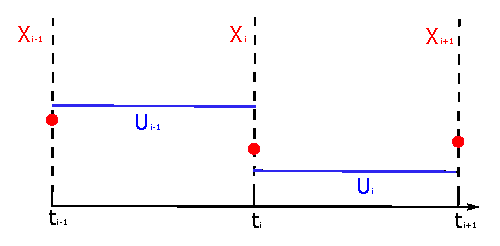
\includegraphics[width=1\textwidth]{MS_int.eps}
	\end{minipage}
	\hfill
	\begin{minipage}{.49\textwidth}
		\centering
		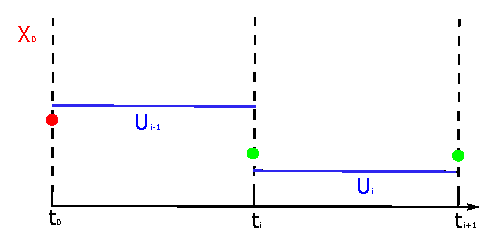
\includegraphics[width=1\textwidth]{SS.eps}
	\end{minipage}
	\caption{Schematic view of the time shooting approaches (left: multiple shooting, right: single shooting).}
	\label{fig:TS}
\end{figure}

In this thesis a multiple shooting approach is used and a Runge-Kutta numerical integration scheme is implemented in order to define the path closing constraints. Runge-Kutta is an explicit integration scheme which has a higher calculation cost than a standard Euler scheme but is more reliable for non-linear systems and has a higher stability with respect to the chosen time step. \cite{Mercy2018}\\ 

It can be noted that the difference between the two shooting approaches is that 'Multiple shooting'(MS) will lead to a larger Hessian of the objective and a larger Jacobian of the constraints. The reason for this is the introduction of more optimization variables. The advantage of MS is then again that these matrices are more sparse because a certain state is only dependent on the previous one and a certain control. Therefore these matrices can be used more efficiently with respect to calculation load. In single shooting every state depends on the begin state and different controls which gives smaller, more densely populated matrices which are more calculation expensive. \cite{Gillis2019}

\section{Model predictive control}
\label{s:MPC_e}
In slow changing environments as for example a chemical plant, MPC is already a mature control technique. More recently this technology also made its introduction in controlling systems with higher dynamics e.g. vehicle control, due to an increase of computational power and the use of more efficiently algorithms. \cite{Mercy2018}. In the next section a short introduction of the formulation is given. \\

During MPC, optimizations are solved in a loop to be able to notice disturbances, changing environments and model-plant mismatch. Therefore it makes use of a moving control horizon\footnote{There are also other implementations e.g. shrinking time horizon, where the control horizon gets smaller every after each iteration.}. Every iteration an OCP is solved starting from the current state and using a certain control horizon.  From the resulting control signals only the first control value is applied for one time interval of the finite control horizon $N\cdot T_{s}$ as is visualized in Figures \ref{fig:MPC1}and \ref{fig:MPC2}.\\
The decision on the amount of samples $N$ that are used in the control horizon is based on a tradeoff between higher accuracy and calculation effort. \cite{TongDuySon2019, Mercy2018}. In Figure \ref{fig:MPC1} the solving of an OCP during one MPC iteration on time sample $t+1$ is depicted. Figure \ref{fig:MPC2} shows that only the first control of the computed control signal will be applied.  This will induces that the system will change its current state. Next a new OCP can be solved. A single OCP-iteration only takes the model of the system into account to calculate the control signals. The iterative way of solving makes the MPC able to deal with unexpected acquired states through feedback that is given by each new current state. As stated earlier the downside of this approach is a bigger computational load, which makes efficiently written software a necessity.  \cite{Patrinos2019}\\

\begin{figure}[h!]
	\centering
	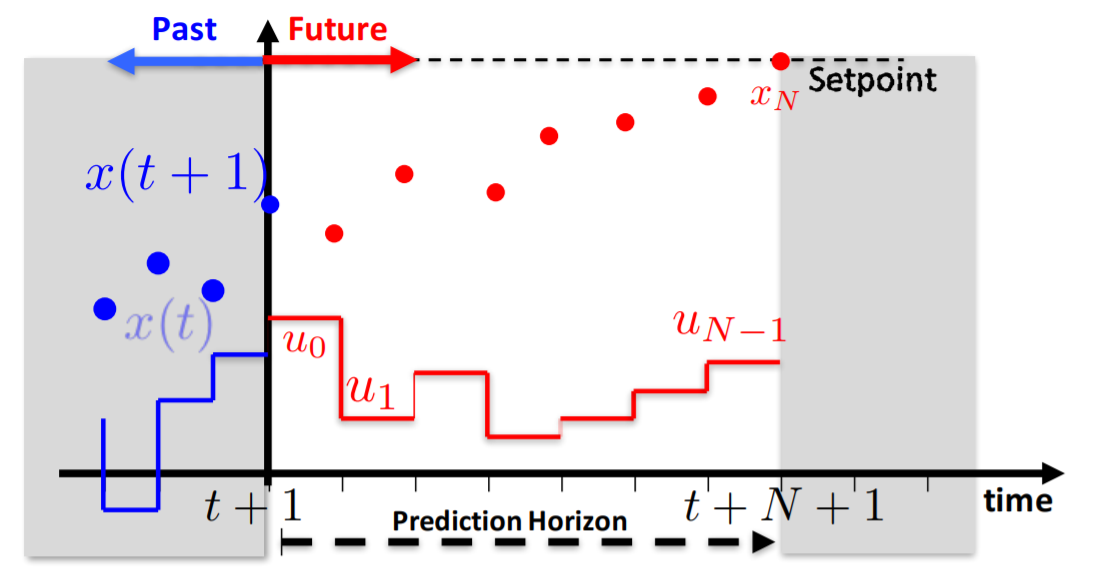
\includegraphics[width=0.6\textwidth]{MPC1.PNG}
	\caption{Visualization of the optimal control problem solved in one iteration of the MPC (Source: \cite{Patrinos2019}).}
	\label{fig:MPC1}
\end{figure}

\begin{figure}[h!]
	\centering
	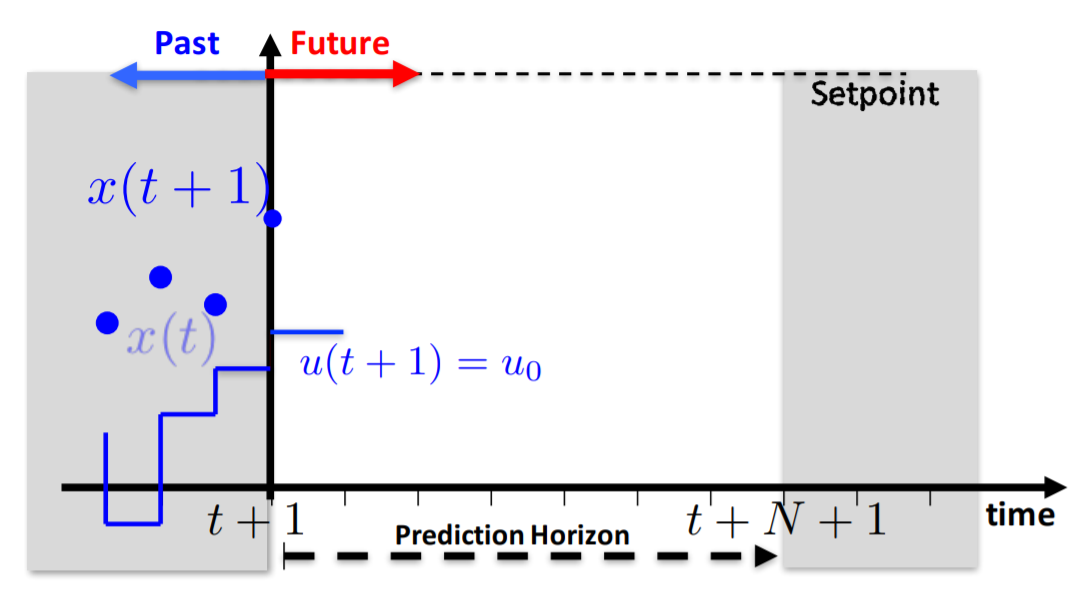
\includegraphics[width=0.6\textwidth]{MPC2.PNG}
	\caption{Visualization of the application of the first step of the calculated control signal during one iteration of the MPC (Source:\cite{Patrinos2019}).}
	\label{fig:MPC2}
\end{figure}


\section{Conclusion}
In this chapter the reader was made acquainted with concepts of optimal control and model predictive control, which will be used in this thesis. 
First a continuous OCP was considered and options how to discretize it were discussed. The option to discretize time best fitted for this thesis, is the "Direct method" together with a multiple shooting approach. It is made sure to take the time step small enough in order to avoid constraint violation. 



%\begin{equation}\label{eq:3}
%minimize_{\bm{q}(.),\bm{u}(.)}\sum_{k = 0}^{N-1}l_{k}(\bm{q}_{k},\bm{u}_{k}) + E(\bm{q}_{N})
%\end{equation}
%\hspace{42 mm} \textit{subject to:}
%\[\bm{\dot{q}}_{k+1} = \sum_{k = 0}^{N-1}\bm{f}(\bm{q}_{k}, \bm{u}_{k})\]
%\[\bm{q}_{0}= \bm{q}_{measured}\]
%\[h(\bm{q}_{k},\bm{u}_{k}) \geq 0\]
%\[\bm{q}_{k}\in Q,\hspace{3 mm} \bm{u}_{k}\in U, \hspace{3 mm} N \in \mathbb{N}\]




%%% Local Variables: 
%%% mode: latex
%%% TeX-master: "thesis"
%%% End: 